\documentclass[a0paper,portrait]{baposter}



\usepackage{wrapfig}
\usepackage{lmodern}

\usepackage[utf8]{inputenc} %unicode support
\usepackage[T1]{fontenc}

\usepackage{tikz} % bullet

\selectcolormodel{cmyk}

\graphicspath{{figures/}} % Directory in which figures are stored


\newcommand{\compresslist}{%
\setlength{\itemsep}{0pt}%
\setlength{\parskip}{1pt}%
\setlength{\parsep}{0pt}%
}

\newcommand{\compresscol}{%
\setlength{\columnsep}{-40pt}%
}

\newenvironment{boenumerate}
  {\begin{enumerate}\renewcommand\labelenumi{\textbf\theenumi.}}
  {\end{enumerate}}

\renewcommand{\labelitemi}{$\bullet$}
\renewcommand{\labelitemii}{$\circ$}
\renewcommand{\labelitemiii}{$\diamond$}
\renewcommand{\labelitemiv}{$\ast$}

\usepackage[font=small,labelfont=bf]{caption}
\usepackage{multirow}
\usepackage{multicol}

\begin{document}


\definecolor{darkblue}{rgb}{0.0, 0.0, 1.0}
\definecolor{lightblue}{rgb}{0.0, 0.5, 1.0}

\begin{poster}
{
grid=false,
headerborder=open, % Adds a border around the header of content boxes
colspacing=1em, % Column spacing
bgColorOne=white, % Background color for the gradient on the left side of the poster
bgColorTwo=white, % Background color for the gradient on the right side of the poster
borderColor=darkblue, % Border color
headerColorOne=lightblue, % Background color for the header in the content boxes (left side)
headerColorTwo=lightblue, % Background color for the header in the content boxes (right side)
headerFontColor=white, % Text color for the header text in the content boxes
boxColorOne=white, % Background color of the content boxes
textborder=rounded, %rectangle, % Format of the border around content boxes, can be: none, bars, coils, triangles, rectangle, rounded, roundedsmall, roundedright or faded
eyecatcher=true, % Set to false for ignoring the left logo in the title and move the title left
headerheight=0.11\textheight, % Height of the header
headershape=rounded, % Specify the rounded corner in the content box headers, can be: rectangle, small-rounded, roundedright, roundedleft or rounded
headershade=plain,
headerfont=\Large\textsf, % Large, bold and sans serif font in the headers of content boxes
%textfont={\setlength{\parindent}{1.5em}}, % Uncomment for paragraph indentation
linewidth=2pt, % Width of the border lines around content boxes
columns=6 
}
{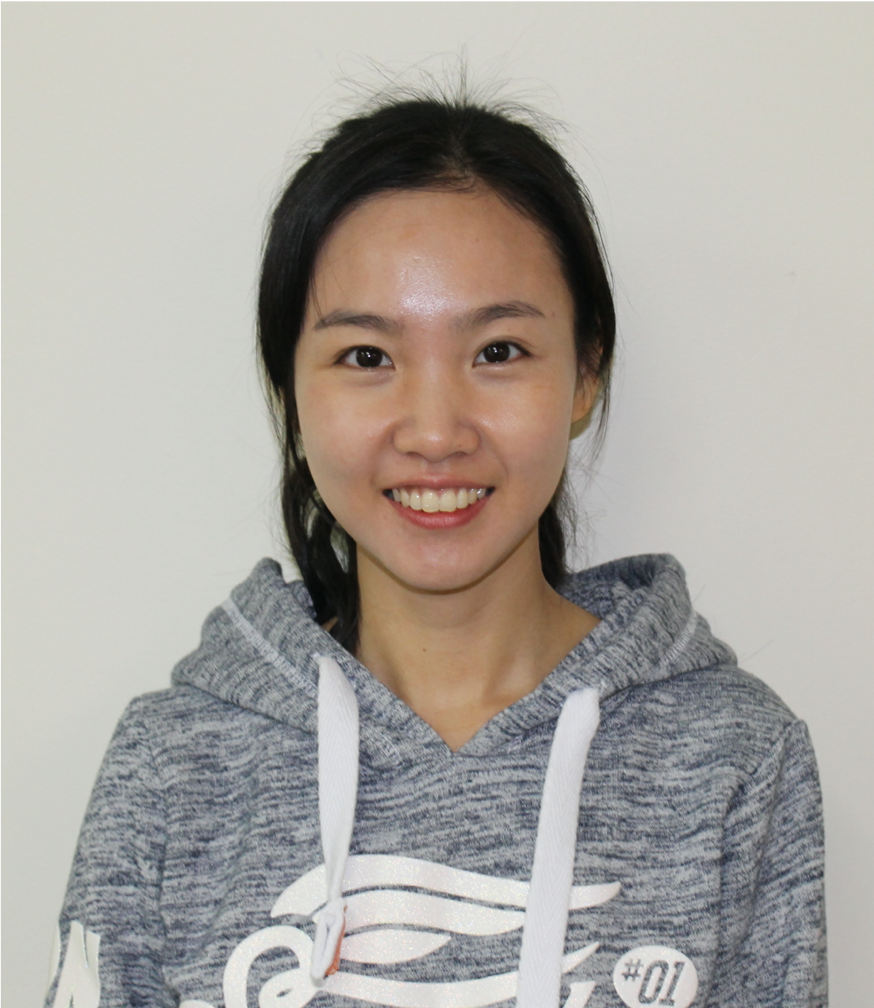
\includegraphics[width=0.12\textwidth]{me.png}}
%
%----------------------------------------------------------------------------------------
%	TITLE AND AUTHOR NAME
%----------------------------------------------------------------------------------------
%
{
\textsf %Sans Serif
{\huge Latent Variable-Based Multivariate Methods to \\[0.1in]
Correct for Batch Effects in Microbiome Data
}
} % Poster title
% {\vspace{1em} Marta Stepniewska, Pawel Siedlecki\\ % Author names
% {\small \vspace{0.7em} Department of Bioinformatics, Institute of Biochemistry and Biophysics, PAS, Warsaw, Pawinskiego 5a}} % Author email addresses
{\sf\vspace{0.5em}
Yiwen Wang\textsuperscript{*} and Kim-Anh L\^e Cao
\vspace{0.1em}\\
\small{Melbourne Integrative Genomics, School of Mathematics and Statistics, University of Melbourne
\vspace{0.2em}\\
\textsuperscript{*} \textbf{email:} yiwenw5@student.unimelb.edu.au | \textbf{twitter:} {\color{cyan} $@$YiwenWang\_Eva}}
}
{
\includegraphics[width=0.1\textwidth]{logo.jpeg}} % University/lab logo 

\small
\headerbox{Introduction}{name=introduction,column=0,row=0, span=6}{
\smallskip 
In the past years, microbial research has made enormous progress with the advent of sequencing technologies to investigate the roles of all microorganisms in different ecological habitats. However, microbiome studies based on 16S amplicon or shotgun sequencing are difficult to replicate as they may suffer from different sources of batch effects. In this context, we define ``\textbf{batch effect}'' as any unwanted source of variation that is unrelated to, and obscures the biological factor of interest. Such batch effects may range from biological to technical and computational factors. Traditional statistical methods developed for microarray or RNA-seq data are generally not suitable for batch effect correction in microbiome data because of the data characteristics. We propose two novel computational methods, PLSDA-batch and sPLSDA-batch based on the Partial Least Squares Discriminant Analysis regression (PLSDA) which take these characteristics into consideration. On real microbiome data, we show that our approaches are robust in removing batch variation while preserving treatment variation compared to existing correction methods. In addition, sPLSDA-batch selects discriminative variables while correcting the batch effects.
 \smallskip
}

%Data are transformed with centered log ratio to account for uneven library sizes and compositional constraints. Both methods are non-parametric and can handle the skewed distribution caused by sparsity and overdispersion. Their multivariate property accounts for the data correlation structure. 

\headerbox{1. Data characteristics }{name=char,column=0,below=introduction,span=3}{


\begin{itemize}

    	\item[$\bullet$] Sparse, overdispersed \\
    	{\color{cyan} $\rightarrow$ {\small skewed and non-Gaussian distribution}}
	\vspace*{-1mm}
    	\item[$\bullet$] Uneven library sizes \\
    	{\color{cyan} $\rightarrow$ {\small bias, difficult to compare samples}}
  	\vspace*{-1mm}
    	\item[$\bullet$] Compositional structure  \\
    	{\color{cyan} $\rightarrow$ {\small relative abundance, hence data are bounded}}
	\vspace*{-1mm}
    	\item[$\bullet$] Microbial variables are not independent 

    \end{itemize}	
}


\headerbox{2. Limitations of existing methods}{name=exist,column=0,below=char,span=3}{

\begin{minipage}{\linewidth}\compresscol
\begin{itemize}
	\item[$\bullet$] ComBat (\textit{sva} package)
	\vspace*{-1mm}
    	\begin{itemize}
    		\item[$\bullet$] {\small Does not consider the correlation between microbial variables}
		\vspace*{-1mm}
    		\item[$\bullet$] {\small Assumes Gaussian distribution}
    	\end{itemize}
	
	\vspace*{-1mm}
	
    	\item[$\bullet$] RUVIII (\textit{ruv} package)
	\vspace*{-1mm}
    	\begin{itemize}
    		\item[$\bullet$] {\small Requires sample replicates}
		\vspace*{-1mm}
    		\item[$\bullet$] {\small Requires negative control variables}
    	\end{itemize}
\end{itemize}
\end{minipage} \\[0.06in]

}

\headerbox{3. PLSDA-batch}{name=plsda,span=3,column=0,below=exist, above=bottom}{ % To reduce this block to 1 column width, remove 'span=2'

\begin{minipage}{\linewidth}
  \centering
  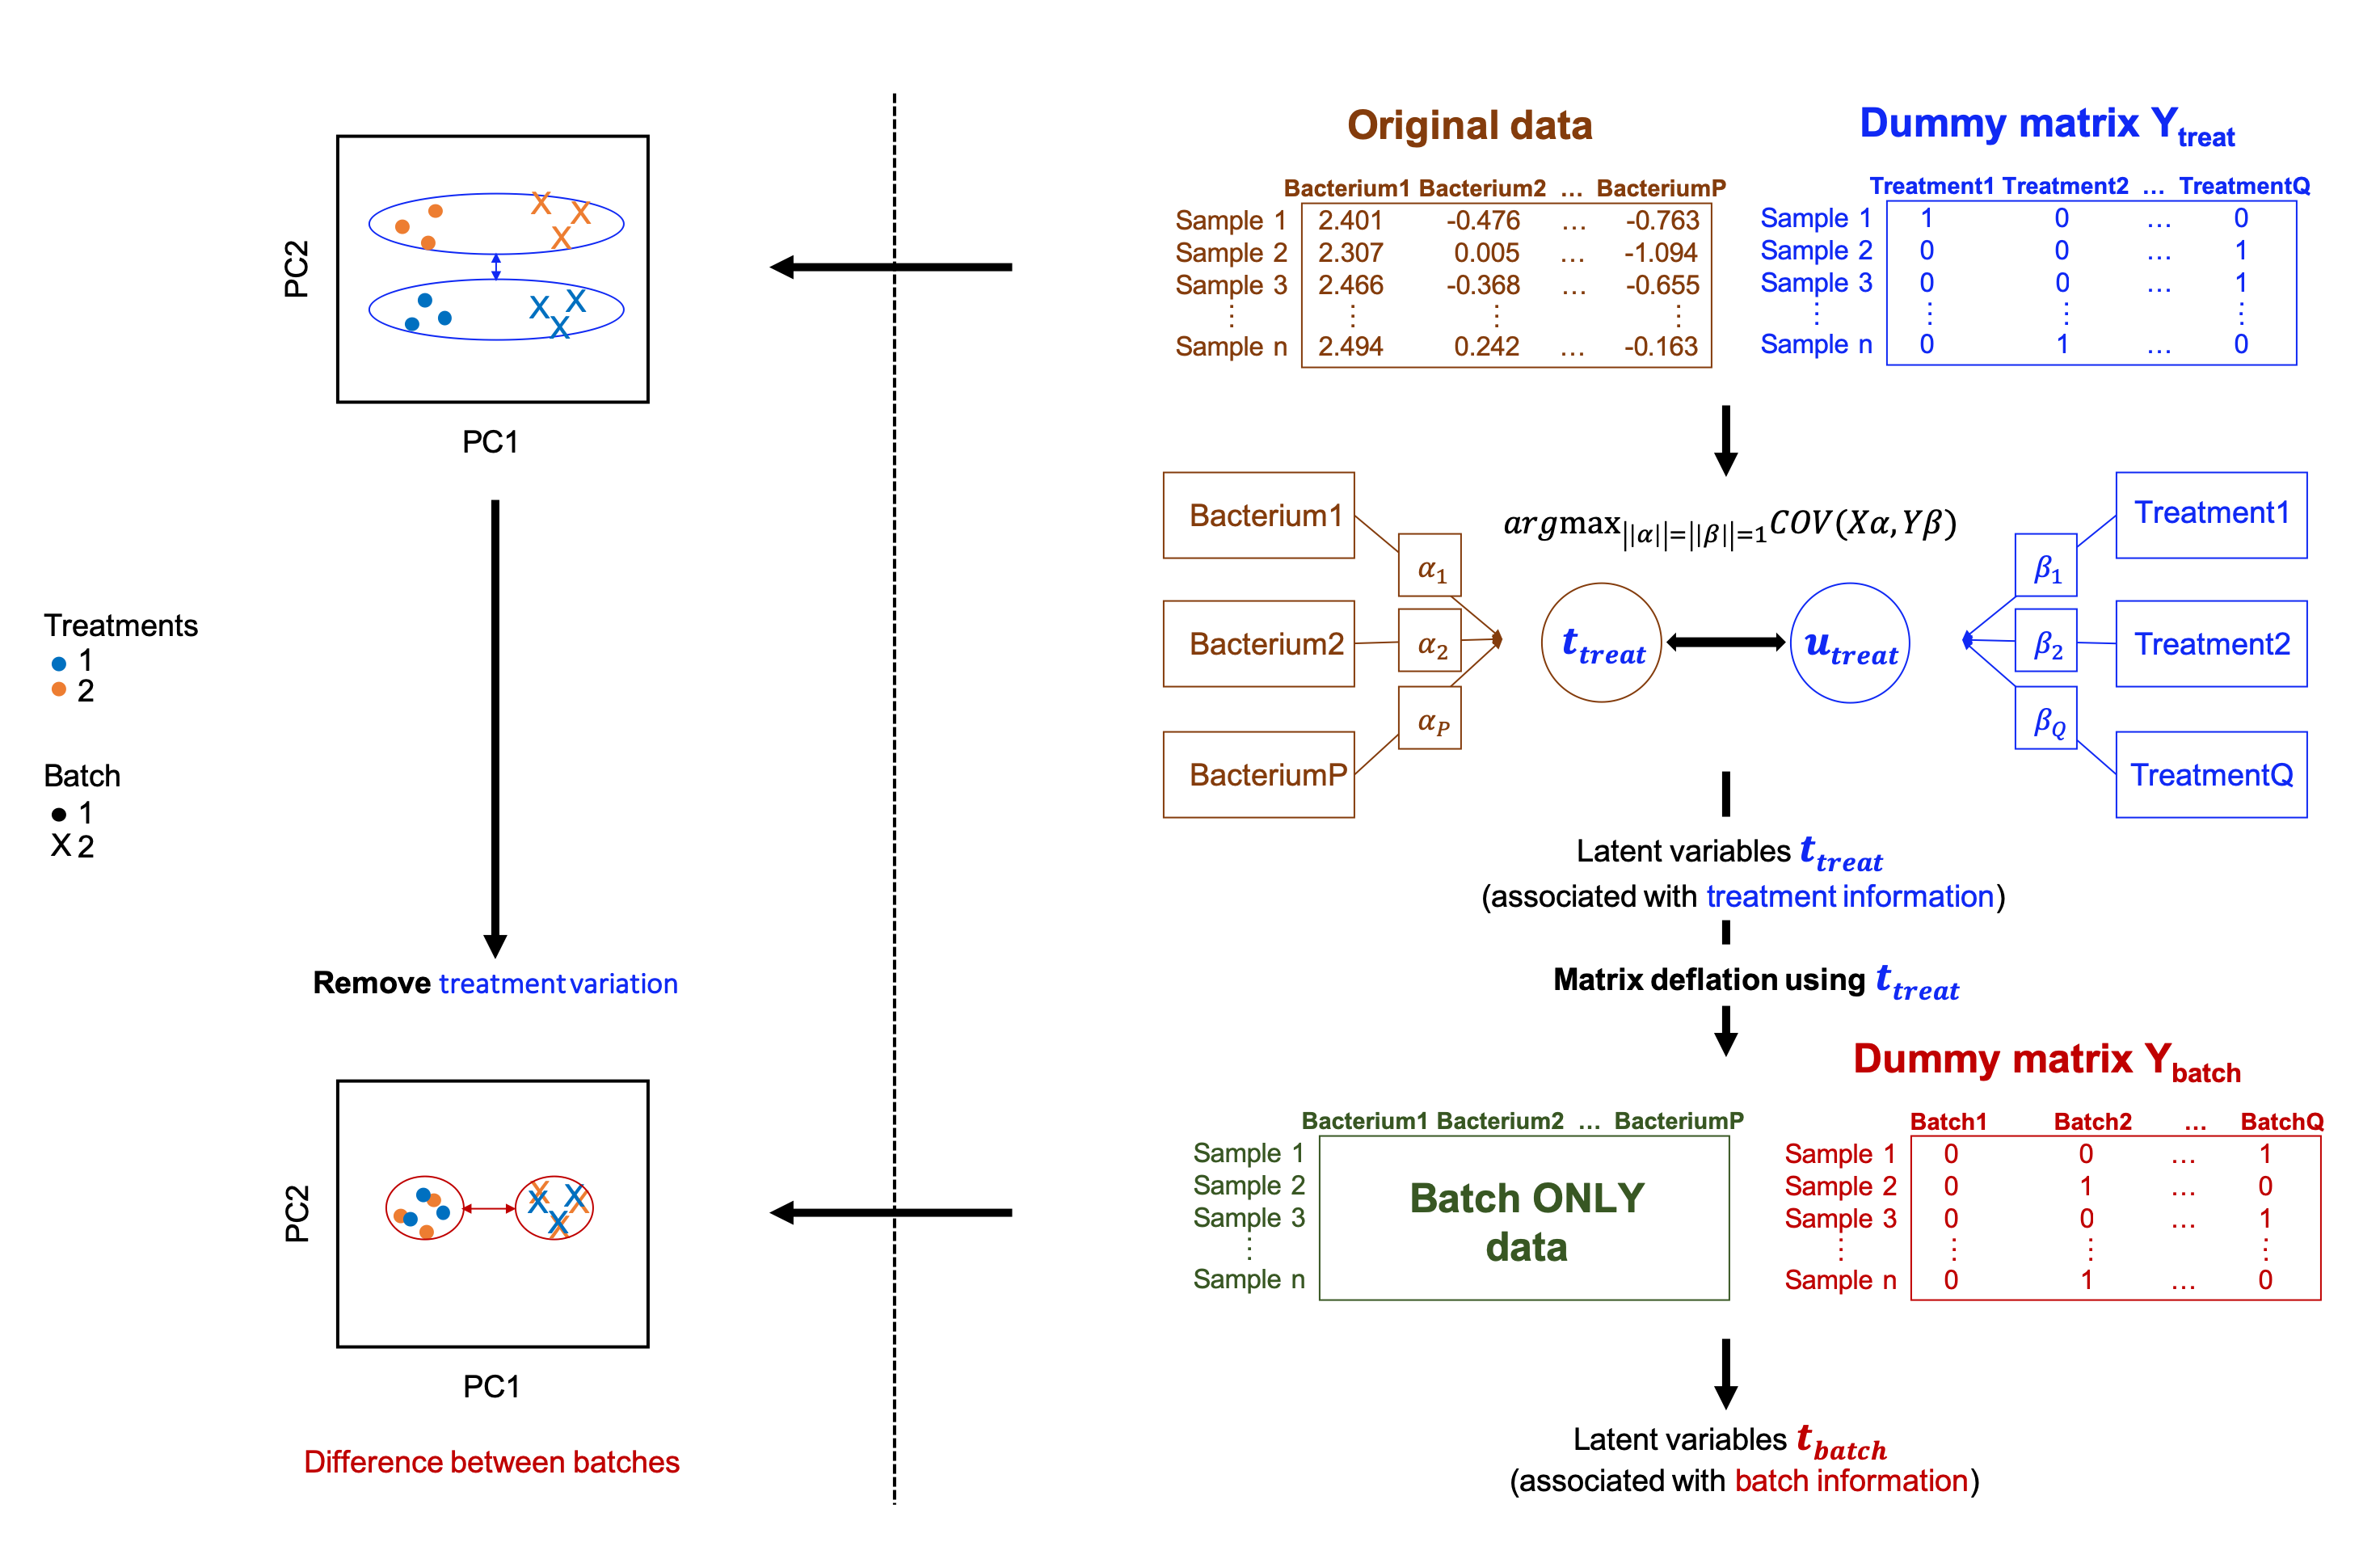
\includegraphics[width=\linewidth]{method1.png}
  \captionof{figure}{\small {\textbf{\textit{Step1:}} estimating the latent variables associated with batch effects}}
  \label{fig:plsda1}
\end{minipage}

\vspace*{3mm}

\begin{minipage}{\linewidth}
  \centering
  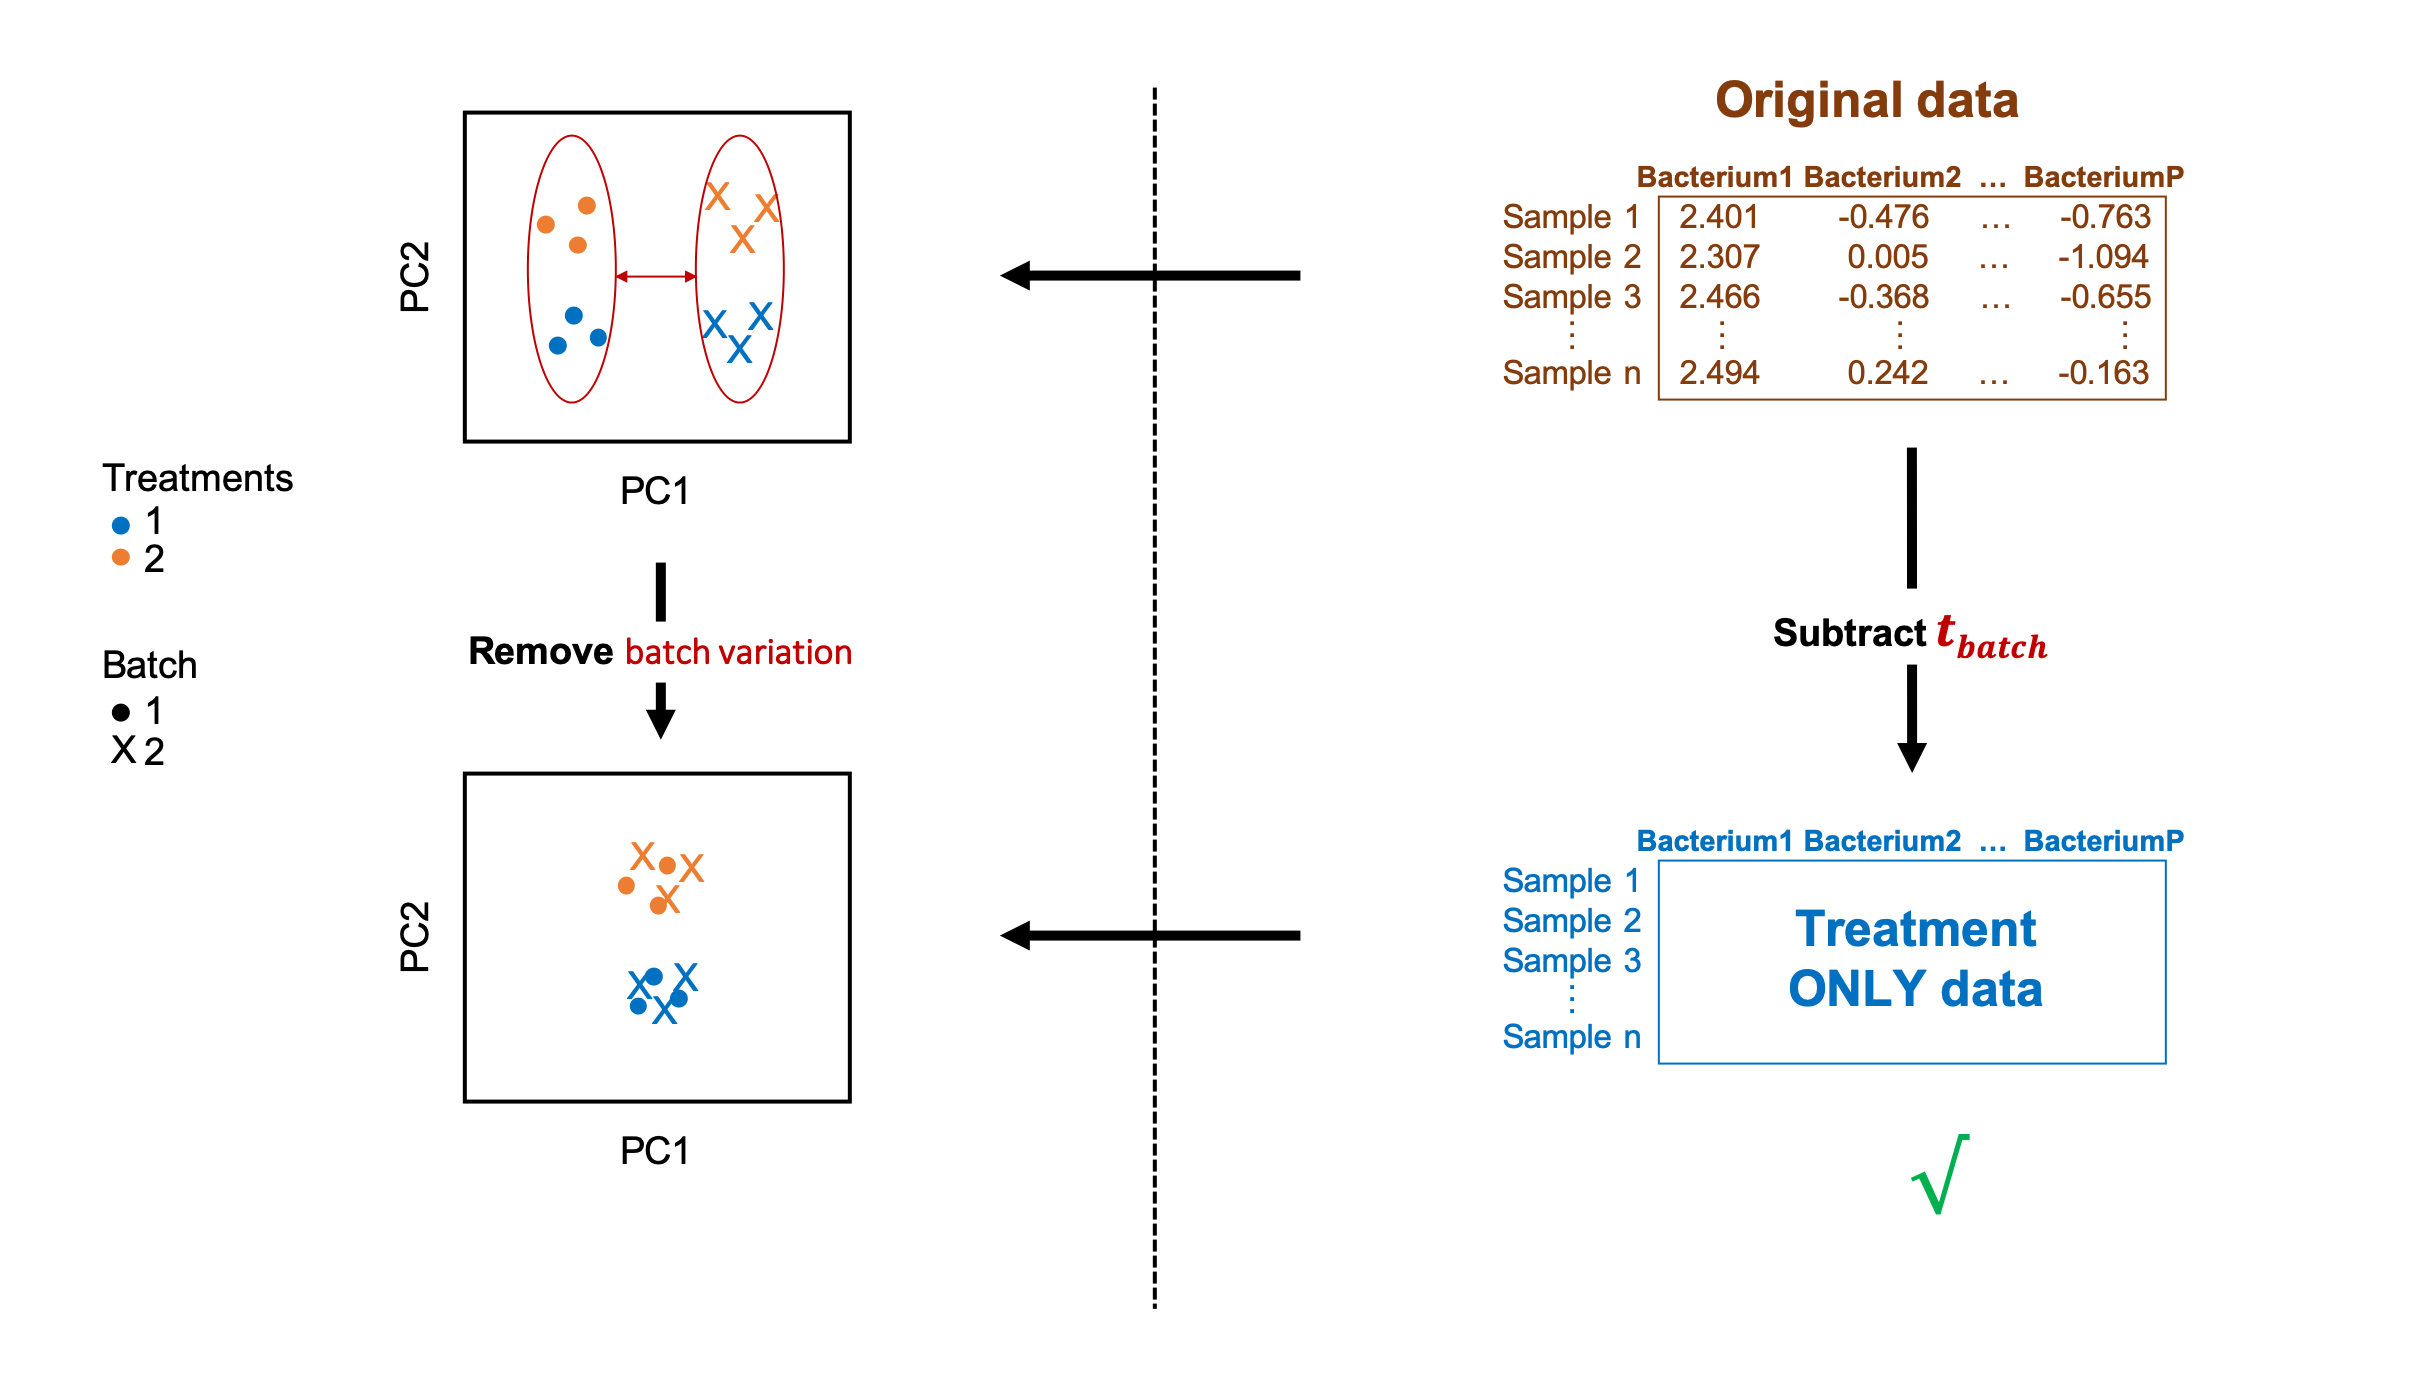
\includegraphics[width=\linewidth]{method2.png}
  \captionof{figure}{\small {\textbf{\textit{Step2:}} removing the latent variables associated with batch effects}}
  \label{fig:plsda2}
\end{minipage}
}


\headerbox{4. sPLSDA-batch}{name=splsda,span=3,column=3,below=introduction}{ 

%Batch effects can be assessed with visualisation and variance calculation, before and after adjustment. 


\begin{minipage}{\linewidth}
Adds constraint to select subsets of microbial variables: 
	\vspace*{-1mm}
	\begin{itemize}
		\item {\small Only removes batch variation from selected variables that discriminate batches} \\
		{\color{cyan} $\rightarrow$  {\small preserves more non-batch variation compared to PLSDA-batch}}
		\vspace*{-1mm}
		\item {\small Selects variables that discriminate treatments} \\
		{\color{cyan} $\rightarrow$  {\small feature selection}}
	\end{itemize}
\end{minipage}

}

\headerbox{5. Managing data characteristics}{name=manage,span=3,column=3,below=splsda}{ 

%Batch effects can be assessed with visualisation and variance calculation, before and after adjustment. 


\begin{minipage}{\linewidth}
 	\begin{itemize}
	\item[$\bullet$] Data are {\color{cyan} Centered Log Ratio} transformed to account for uneven library sizes and compositional constraints. \\
	\vspace*{-4mm}
	\item[$\bullet$] PLSDA-batch \& sPLSDA-batch are {\color{cyan} non-parametric}: Can handle skewed distributions caused by sparsity and overdispersion. \\
	\vspace*{-4mm}
	\item[$\bullet$] Their multivariate property accounts for the data correlation structure. \\
	\end{itemize}
	\vspace*{-4mm}
\end{minipage}

}


\headerbox{6. Case study}{name=case,column=3,below=manage,span=3}{

\begin{minipage}{\linewidth}
\centering
\small
\begin{tabular}{cc}
\hline
                   & \textbf{Anaerobic digestion} \\ \hline
No. of microbial variables       & 231                                        \\
No. of samples     & 28                                         \\
Factor of interest & {\color{cyan} Phenol concentration}               \\
Batch sources      & {\color{cyan} Sequencing dates}                     \\ \hline
\end{tabular}

%\flushright
%\vspace*{-5mm}
%{\tiny (Chapleur \textit{et al}, 2016)}
\end{minipage} \\[0.07in]

}






\headerbox{7. Results}{name=res,span=3,column=3,below=case}{ 

%Batch effects can be assessed with visualisation and variance calculation, before and after adjustment. 



\begin{multicols}{2}
\begin{minipage}{\linewidth}
 \centering
 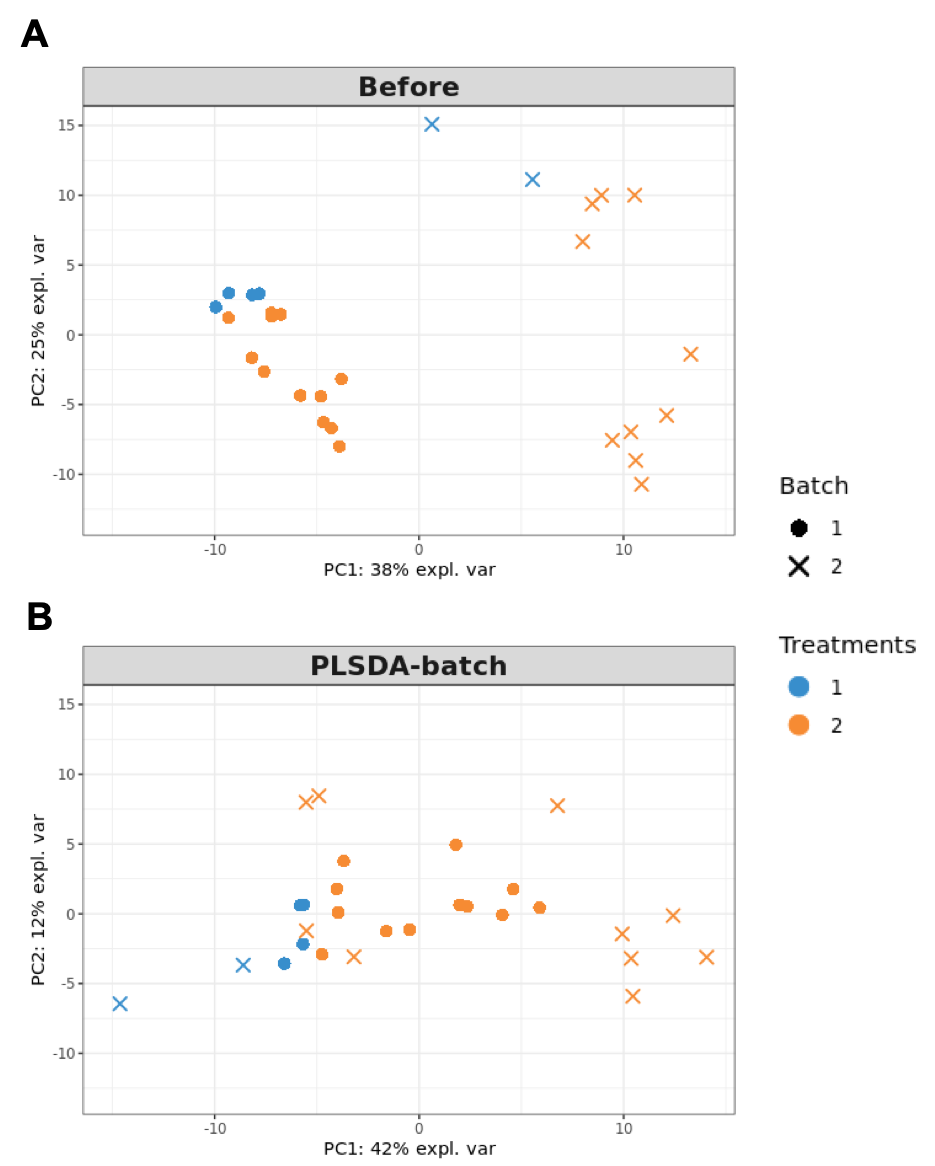
\includegraphics[width=\linewidth]{res1.png}
 \vspace*{0.5mm}
\end{minipage}

\begin{minipage}{\linewidth}
 \centering
 \vspace*{6mm}
 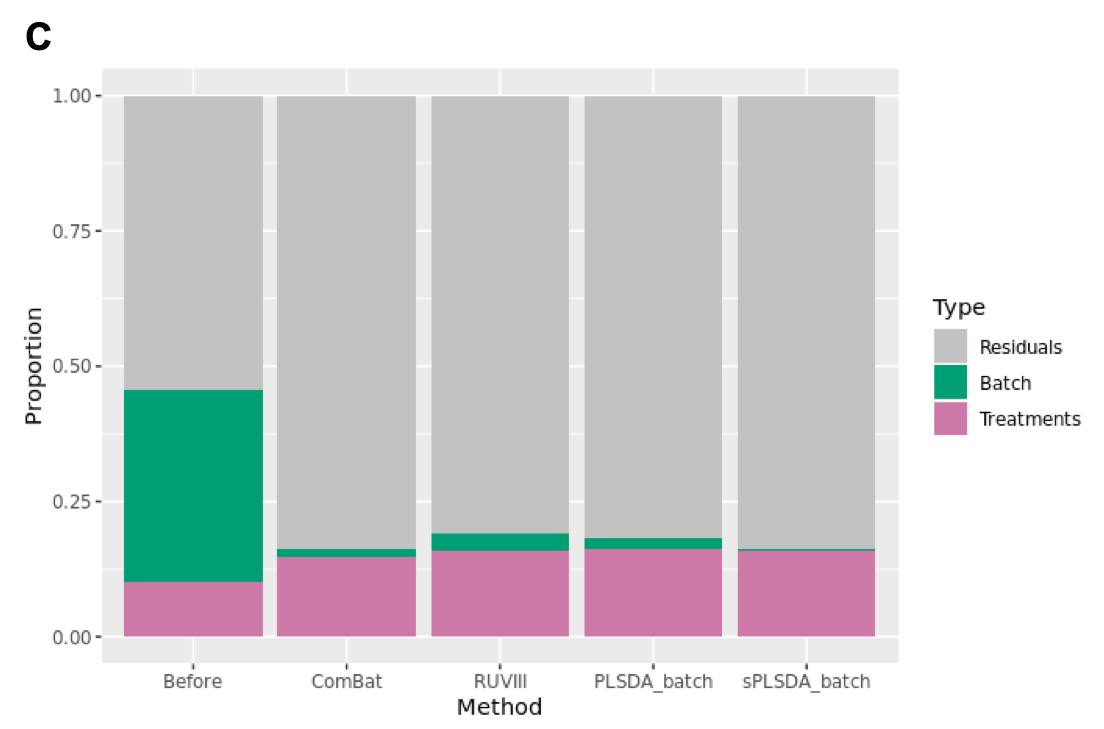
\includegraphics[width=\linewidth]{res2.png}
 
 \captionof{figure}{
  \scriptsize{
 PCA sample plots before  \textbf{(A)}  and after \textbf{(B)}  PLSDA-batch correction. Barplots \textbf{(C)} of proportion of variance explained by either batch or factor of interest calculated using partial Redundancy Analysis before and after batch correction with different methods.}}
  
\end{minipage}
\end{multicols}
}


\headerbox{Conclusions}{name=conclusion,column=3,below=res,span=3}{

\begin{minipage}{\linewidth}
{\small
\begin{itemize}%\compresslist
	\item[$\bullet$] PLSDA-batch \& sPLSDA-batch remove more batch variation compared to RUVIII, revealing more variation of interesting effects compared to ComBat.
	\vspace*{-2mm}
	\item[$\bullet$] sPLSDA-batch selects discriminative variables while removing batch effects.
	\vspace*{-2mm}
	\item[$\bullet$] Limitation: batch effects strongly confounded with treatment effects cannot be corrected for in microbiome studies.
	\vspace*{-2mm}
	\item[$\bullet$] We have validated our methods on simulated data and will work with collaborators to interpret the microbial signature biologically.
\end{itemize}
}
\end{minipage} \\[0.03in]


}

\headerbox{Acknowledgements}{name=ack,column=3,below=conclusion,span=3,above=bottom}{
\footnotesize
\begin{minipage}[b]{0.22\linewidth}
    
\includegraphics[width=1\textwidth]{logo_fund.pdf}
\end{minipage}%
\hfill
\begin{minipage}[b]{0.75\linewidth}%
NHMRC Career Development Fellowship CDF1 GNT1087415 (KALC) and China Scholarship Council (CSC) PhD scholarship (YW).
\end{minipage}
}

%\headerbox{References}{name=references,column=3,span=3,below=evaluation,above=bottom}{

%\small % Reduce the font size in this block
%\renewcommand{\section}[2]{\vskip 0.05em} % Get rid of the default "References" section title
%\nocite{*} % Insert publications even if they are not cited in the poster

%\bibliographystyle{plain}
%\bibliography{poster} % Use sample.bib as the bibliography file
%}

\end{poster}

\end{document}
